\documentclass[12pt]{beamer}
\usetheme{Boadilla}
\usepackage{tikz}
\renewcommand{\arraystretch}{1.25}
\usetikzlibrary{trees}
\title[ECON2843]{ECON2843 Elements of Statistics}
\subtitle{Part 1 Descriptive Statics, Summary Measures, and Data Visualization}
\date{}
\usepackage{amsmath,amssymb,mathtools,wasysym}
\begin{document}
\begin{frame}
	\titlepage
\end{frame}
\section{Introduction}
\begin{frame}{Roadmap for Course}
	First half of course - learn some fundamental statistical concepts and tools:
		\begin{itemize}
			\item[$\triangleright$] Descriptive statistics for data
			\item[$\triangleright$] Summary measures
			\item[$\triangleright$] Data visualization
			\item[$\triangleright$] Probability
			\item[$\triangleright$] Probability distributions
			\item[$\triangleright$] Sampling and sampling distributions
			\item[$\triangleright$] etc..
		\end{itemize}
\end{frame}
\begin{frame}{Roadmap for Course}
	Second half of course - use the tools and techniques from first half to tackle more complex statistical questions:
	\begin{itemize}
		\item[$\triangleright$] Estimation
		\item[$\triangleright$] Test a hypothesis
		\item[$\triangleright$] Compare two distributions: $\chi$-square test; analysis of variance
		\item[$\triangleright$] Correlation and regression
		\item[$\triangleright$] Applications
		\item[$\triangleright$] etc..
	\end{itemize}
\end{frame}
\begin{frame}{I have a Question...}
	\begin{itemize}
		\item[$\blacktriangleright$] I ask myself at night, "Am I smarter than the average person?"
		\item[$\blacktriangleright$] How can I find out?
	\end{itemize}
\end{frame}
\begin{frame}{I have a Question...}
	\begin{itemize}
		\item[$\blacktriangleright$] Step 1: Establish a relevant variable of interest.
		\begin{itemize}
			\item Perhaps IQ might be appropriate.
		\end{itemize}
		\item[$\blacktriangleright$] Step2: Compare my IQ to a benchmark.
		\begin{itemize}
			\item How do we form this benchmark?
			\item We need to think back to the original question.
		\end{itemize}
	\end{itemize}
\end{frame}
\begin{frame}{I have a Question...}
	\begin{itemize}
		\item[$\blacktriangleright$] A good benchmark might be the average IQ in the population.
		\item[$\blacktriangleright$] Ideal setting is to survey everyone on the planet and calculate the average IQ.
		\item[$\blacktriangleright$] In practice, this is impossible.
		\item[$\blacktriangleright$] What to do?
	\end{itemize}
\end{frame}
\begin{frame}{I have a Question...}
	\begin{itemize}
		\item[$\blacktriangleright$] Use a (representative) sample from the population.
		\item[$\blacktriangleright$] Compare my IQ to the average IQ of the sample.
		\item[$\blacktriangleright$] Then, answer my original question.
	\end{itemize}
\end{frame}
\begin{frame}{The Study of Statistics}
	To summaries we
	\begin{itemize}
		\item[$\blacktriangleright$] Established a question of interest, or {\sl\color{red} hypothesis}, that can be tested.
		\item[$\blacktriangleright$] Determine some relevant {\sl\color{red} variables}.
		\item[$\blacktriangleright$] Identified our {\sl\color{red} population} of interest.
		\item[$\blacktriangleright$] Gathered some data by taking a {\sl\color{red} sample} from the population.
		\item[$\blacktriangleright$] Analyze the data we gathered.
		\item[$\blacktriangleright$] Form a {\sl\color{red}causal inference} or conclusion regarding the original hypothesis.
	\end{itemize}
\end{frame}
\begin{frame}{The Study of Statistics}
	\begin{itemize}
		\item[$\blacktriangleright$] Statistics is essentially the study of {\bf data}.
		\item[$\blacktriangleright$] More specifically, {\bf statistical inference} refers to the problem of determining the behavior of a large population by studying a small sample of data from that population.
	\end{itemize}
\end{frame}
\begin{frame}{Terminology and Notation}
	\begin{itemize}
		\item[$\blacktriangleright$] Population: Every observation of interest available in the physical world.\medskip\\
		For example:
		\begin{itemize}
			\item Every single person in Norman, Oklahoma.
			\item Every single student who has ever taken ECON2843.
		\end{itemize}
		\item[$\blacktriangleright$] Usually use $N$ to denote the total number of observations in the population.
	\end{itemize}
\end{frame}
\begin{frame}{Terminology and Notation}
	\begin{itemize}
		\item[$\blacktriangleright$] Populations have {\bf parameters}: A descriptive measure of a population that is usually {\color{red}unobservable} and {\color{red}unknown}. The parameters are characteristic of a population.
		\item[$\blacktriangleright$] Parameters are typically denoted by Greek letters:
		\begin{itemize}
			\item Population average/mean: $\mu$
			\item Population variance: $\sigma^2$
		\end{itemize}
	\end{itemize}
\end{frame}
\begin{frame}{Terminology and Notation}
	\begin{itemize}
		\item[$\blacktriangleright$] {\bf Sample}: A selection of observations drawn randomly from the population of interest.\medskip\\
		For example:
		\begin{itemize}
			\item A random sample of 50 OU students from the entire university.
			\item A random sample of 10 ECON2843 students.
		\end{itemize}
		\item[$\blacktriangleright$] Usually use $n$ to denote the total number of observations in the sample.
	\end{itemize}
\end{frame}
\begin{frame}{Terminology and Notation}
	\begin{itemize}
		\item[$\blacktriangleright$] Sample have {\bf statistics}: A descriptive measure of a sample that can be {\color{red}observed (calculated)} and is {\color{red}known}.
		\item[$\blacktriangleright$] Sample statistics are used to make inferences about population parameters and are typically denoted by Roman letters:
		\begin{itemize}
			\item Sample average/mean: $\bar{X}$
			\item Sample variance: $s^2$
		\end{itemize}
	\end{itemize}
\end{frame}

\begin{frame}{Terminology and Notation}
	\begin{itemize}
		\item[$\blacktriangleright$] {\bf Variable}: Any quantity or characteristic that can be measured or recorded for {\sl each observation} in a population or sample.\medskip\\
		For example:
		\begin{itemize}
			\item A person's IQ.
			\item A person's eye color.
			\item A stock's price.
		\end{itemize}
		\item[$\blacktriangleright$] The value of a variable is likely to be different from observation to observation, hence the name variable.
	\end{itemize}
\end{frame}

	\begin{frame}{Types of Data}
	\centering
	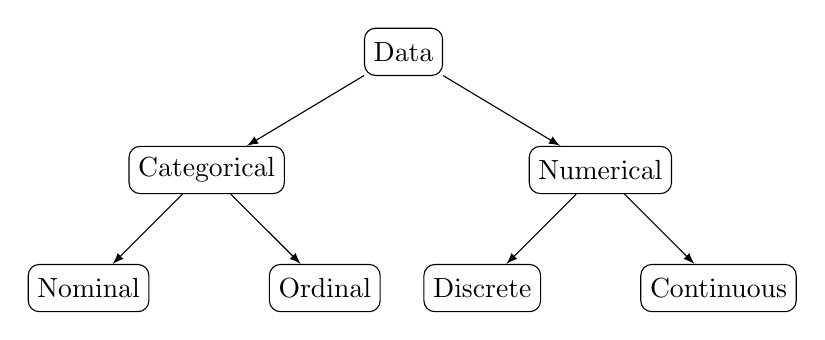
\begin{tikzpicture}[
		level 1/.style={sibling distance=50mm},
		level 2/.style={sibling distance=30mm},
		edge from parent/.style={draw,-latex},
		every node/.style={draw,rounded corners,minimum size=6mm,fill=white,align=center}
		]
		\node {Data}
		child {node {Categorical}
			child {node {Nominal}}
			child {node {Ordinal}}
		}
		child {node {Numerical}
			child {node {Discrete}}
			child {node {Continuous}}
		};
	\end{tikzpicture}
	
\end{frame}

\begin{frame}{Categorical Data}
	\begin{itemize}
		\item[$\blacktriangleright$] Data where the values fall into categories.
		\item[$\blacktriangleright$] Nominal data: The categories have no ordering or relationship.\medskip\\
		Examples: Marital status, eye color, job, etc.
		\item[$\blacktriangleright$] Ordinal data: The categories have a distinct ordering.\medskip\\
		Examples: Ranking teacher performance as "poor/fair/good", survey answer "strongly disagree/disagree/agree/strongly agree", etc.
	\end{itemize}
\end{frame}
\begin{frame}{Descriptive Tools for Categorical Data}
	Numerically:
	\begin{itemize}
	\item[$\blacktriangleright$]Frequency of each category.
	\item[$\blacktriangleright$] {\bf Mode}: The most frequently occurring observation.
	\end{itemize}
	Graphically:
	\begin{itemize}
		\item[$\blacktriangleright$] Bar charts.
		\item[$\blacktriangleright$] Pie charts.
	\end{itemize}
\end{frame}
\begin{frame}{Presentation of Nominal Data: Example}
	\begin{itemize}
		\item[$\blacktriangleright$] Experiment done to determine the favorite colors of students at a university.
		\item[$\blacktriangleright$] We surveyed 206 students and asked the question:What is your favorite color?
	\end{itemize}
\vspace{0.5cm}
\begin{tabular}{|l|c|c|c|c|c|c|c|c|}
	\hline
	Color & Black & Blue & Green & Grey & Purple & Red & White & Other \\
	\hline
	Count & 40 & 43 & 15 & 17 & 15 & 16 & 29 & 31 \\
	\hline
\end{tabular}
\vspace{0.5cm}
\begin{itemize}
	\item[$\blacktriangleright$]  The mode is {\sl\color{blue} blue}, most frequently occurring observation.
\end{itemize}
\end{frame}
\begin{frame}{Presentation of Nominal Data: Example}
%\begin{figure}[h]
\centering
\includegraphics[width=12cm]{bar.png}
%\end{figure}
\end{frame}
\begin{frame}{Presentation of Nominal Data: Example}
%	\begin{figure}[h]
	\centering
	\includegraphics[width=8cm]{pie.png}
%	\end{figure}
\end{frame}
\begin{frame}{Presentation of Ordinal Data}
	\begin{itemize}
	\item[$\blacktriangleright$] Can use exactly the same tools we used for nominal data, e.g., bar charts, pie charts.
	\item[$\blacktriangleright$] But, the most important thing is that we preserve the order of the categories.
	\item[$\blacktriangleright$] But, the most important thing is that we preserve the order of the categories.
	For example, the bars in a bar chart should be in increasing or decreasing ordinal value.
\end{itemize}
\end{frame}
\begin{frame}{Time Series vs Cross-Sectional Data}
	
	\begin{itemize}
		\item[$\blacktriangleright$] \textbf{Time Series Data}:
		\begin{itemize}
			\item Data points collected over time.
			\item Each observation corresponds to a different time point.
			\item Example: Daily stock prices, monthly unemployment rates, etc.
		\end{itemize}
		
		\vspace{0.3cm}
		
		\item[$\blacktriangleright$] \textbf{Cross-Sectional Data}:
		\begin{itemize}
			\item Data collected at a single point in time.
			\item Each observation represents a different individual or entity.
			\item Example: GDP of various countries in a given year, employee counts across companies on a specific day, etc.
		\end{itemize}
	\end{itemize}
	
\end{frame}
\begin{frame}{Numerical Data}
	\begin{itemize}
		\item[$\blacktriangleright$] Data where the values can be {\sl measured}.
		\item[$\blacktriangleright$] {\bf Continuous data}: Anything that can be measured in infinitely small increments. Example: Weight, Height, etc.
		\item[$\blacktriangleright$] {\bf Discrete data}: Anything that can be measured in fixed increments.
		\begin{itemize}
		\item The number of cars you own, number of heads in three coin flips, etc.
	    \end{itemize}
	\end{itemize}
\end{frame}
\begin{frame}{To Describe Numerical Data}
Numerically:
		\begin{itemize}
			\item Mean, median, mode.
			\item Quantile.
			\item Range, variance, coefficient of variance.
			\item Covariance, correlation.
		\end{itemize}
Graphically:
\begin{itemize}
	\item Histograms.
	\item Boxplots.
\end{itemize}
\end{frame}

\begin{frame}{Measures of Central Tendency}
	\begin{itemize}
		\item[$\blacktriangleright$] A {\bf measure of central tendency} measures the location of the middle or center of the distribution of your data.
		\item[$\blacktriangleright$] Common measures include the arithmetic mean, the median and the mode.
	\end{itemize}
\end{frame}
\begin{frame}{Measures of Central Tendency}
	\begin{itemize}
		\item[$\blacktriangleright$] Suppose we have two tutorial sessions, A and B.
		\item[$\blacktriangleright$] We would like to establish which tutorial session performed better in a recent quiz:
	\end{itemize}
	\vspace{0.5cm}
	\centering
	\begin{tabular}{|c|c|c|c|c|c|c|c|c|}
		\hline
		A & 5 & 6 & 5 & 7 & 8 & 7 & 8 & 8\\
		\hline
		B & 9 & 5 & 6 & 7 & 7 & 6 & 5 & \\
		\hline
	\end{tabular}
\end{frame}
\begin{frame}{Mean}
	\begin{itemize}
		\item[$\blacktriangleright$] The {\bf arithmetic mean} is the average of all the observations.
		\item[$\blacktriangleright$] Population mean:
		$$\mu=\frac{1}{N}(X_1+\cdots+X_N)=\frac{1}{N}\sum_{i=1}^NX_i$$
		\item[$\blacktriangleright$] Sample mean:
		$$\bar{X}=\frac{1}{n}(X_1+\cdots+X_n)=\frac{1}{n}\sum_{i=1}^nX_i$$
	\end{itemize}
\end{frame}
\begin{frame}{Mean}
	So for the two tutorial sessions:
\vspace{0.5cm}
	
\begin{center}
	\begin{tabular}{|c|c|c|c|c|c|c|c|c|}
		\hline
		A & 5 & 6 & 5 & 7 & 8 & 7 & 8 & 8\\
		\hline
		B & 9 & 5 & 6 & 7 & 7 & 6 & 5 & \\
		\hline
	\end{tabular}
    
\end{center}
\vspace{0.5cm}
	
	Tutorial A: The mean of students' grades is 6.75.
	
	Tutorial B: The mean of students' grades is 6.43.
\end{frame}
\begin{frame}{Median}
	The median is the middle observation. Rank the observations in ascending order; median is the middle observation if $n$ is odd, or the average of the middle two observations if $n$ is even.
	\vspace{0.5cm}
	
	\begin{center}
		\begin{tabular}{|c|c|c|c|c|c|c|c|c|}
			\hline
			A & 5 & 6 & 5 & 7 & 8 & 7 & 8 & 8\\
			\hline
			B & 9 & 5 & 6 & 7 & 7 & 6 & 5 & \\
			\hline
		\end{tabular}
	\end{center}
	\vspace{0.5cm}
	
	Tutorial A: The median is ?
	
	Tutorial B: The median is ?
\end{frame}
\begin{frame}{Mode}
	The mode is the most frequently occurring observation.
	\vspace{0.5cm}
	
	\begin{center}
		\begin{tabular}{|c|c|c|c|c|c|c|c|c|}
			\hline
			A & 5 & 6 & 5 & 7 & 8 & 7 & 8 & 8\\
			\hline
			B & 9 & 5 & 6 & 7 & 7 & 6 & 5 & \\
			\hline
		\end{tabular}
	\end{center}
	\vspace{0.5cm}
	
	Tutorial A: The mode is ?
	
	Tutorial B: The mode is ?
\end{frame}
\begin{frame}{Mean vs Median}
	The mean is the most commonly used measure.
	
	\vspace{0.5cm}
	
	But, the median is more robust to extreme observations.
	
	\begin{center}
		\begin{tabular}{|c|c|c|c|c|c|c|c|}
			\hline
			B & 9 & 5 & 6 & 7 & 7 & 6 & 5\\
			\hline
		\end{tabular}
	\end{center}
	
	Mean = 6.43, median = 6.
	\vspace{0.5cm}
	
	\begin{center}
	\begin{tabular}{|c|c|c|c|c|c|c|c|}
		\hline
		B &90 & 5 & 6 & 7 & 7 & 6 & 5\\
		\hline
	\end{tabular}
	\end{center}
	
	Mean = 18, median = 6.
\end{frame}
\begin{frame}{Measures of Variability}
Let's say we receive the final grades for the semester for students in the two tutorial sessions:

\vspace{0.5cm}

\begin{center}
	\begin{tabular}{|c|c|c|c|c|c|c|c|c|}
		\hline
		A & 75& 80 & 70 & 77 & 73 & 75 & 90 & 60\\
		\hline
		B & 75 & 100 & 50 & 85 & 65 & 98 & 52 & \\
		\hline
	\end{tabular}
\end{center}
\end{frame}
\begin{frame}{Measures of Variability}
	If we calculate the mean of each tutorial, we find that they are both equal to 75.
	
	\begin{center}
		\begin{tabular}{|c|c|c|c|c|c|c|c|c|c|}
			\multicolumn{10}{r}{$\bar{X}$} \\ 
			\hline
			A & 75& 80 & 70 & 77 & 73 & 75 & 90 & 60&75\\
			\hline
			B & 75 & 100 & 50 & 85 & 65 & 98 & 52 &&75\\
			\hline
		\end{tabular}
	\end{center}
\end{frame}
\begin{frame}{Measures of Variability}
	\begin{itemize}
		\item[$\blacktriangleright$] However, it is clear that these two tutorials are not the same.
		\item[$\blacktriangleright$] Is there another characteristic of the distributions of marks that we can measure and compare?
		\item[$\blacktriangleright$] Variability!
		\begin{itemize}
		\item Which tutor is more consistent in their teaching methods?
		\end{itemize}
		\item[$\blacktriangleright$] How can we quantify the difference in variability or "spread" in the marks?
	\end{itemize}
\end{frame}
\begin{frame}{Range}
	\begin{itemize}
		\item[$\blacktriangleright$] The range of a data set is defined to be:
		
		\vspace{0.5cm}
		Range $=$ Largest Value $-$ Smallest Value
		
		\vspace{0.5cm}
		\item[$\blacktriangleright$] Session A: The range is $90- 60 = 30$.
		\item[$\blacktriangleright$] Session B: The range is $100-50 = 50$.
		\item[$\blacktriangleright$] Range is simple to understand and calculate, but can be affected by extreme observations or "outliers".
	\end{itemize}
\end{frame}
\begin{frame}{Measures of Variability}
	\begin{itemize}
		\item[$\blacktriangleright$] The range is useful, but it is calculated using only two numbers.
		\item[$\blacktriangleright$] What about the other observations in our data set?
		\item[$\blacktriangleright$] A better idea for measuring the variability might be to look at the distance of each observation from a central measure...
	\end{itemize}
\end{frame}
\begin{frame}{Measures of Variability}
	\begin{itemize}
		\item[$\blacktriangleright$]Distances from the mean, i.e., $(X_i-\bar{X})$.
	\end{itemize}
	\begin{center}
		\begin{tabular}{|c|c|c|c|c|c|c|c|c|c|}
			\hline
			\multicolumn{9}{|c|}{$X_i$} & $\bar{X}$\\ \hline
			\hline
			A & 75& 80 & 70 & 77 & 73 & 75 & 90 & 60&75\\
			\hline
			B & 75 & 100 & 50 & 85 & 65 & 98 & 52 &&75\\
			\hline
		\end{tabular}
		
		\vspace{0.5cm}
		
		\begin{tabular}{|c|c|c|c|c|c|c|c|c|c|}
			\hline
			\multicolumn{9}{|c|}{$X_i-\bar{X}$} & $\sum$\\ \hline
			\hline
			A & 0& 5 & $-5$ & 2 & $-2$ & 0 & 15 & $-15$&0\\
			\hline
			B & 0 & 25 & $-25$ & 10 & $-10$ & 23& $-23$ &&0\\
			\hline
		\end{tabular}
	\end{center}
\end{frame}
\begin{frame}{Measures of Variability}
	\begin{itemize}
		\item[$\blacktriangleright$]Squared distances from the mean, i.e., $(X_i-\bar{X})^2$.
	\end{itemize}
	\begin{center}
		\begin{tabular}{|c|c|c|c|c|c|c|c|c|c|}
			\hline
			\multicolumn{9}{|c|}{$(X_i-\bar{X})^2$} & $\sum$\\ \hline
			\hline
			A & 0& 25 & 25 & 4 & 4 & 0 & 225 & 225&508\\
			\hline
			B & 0 & 625 & 625 & 100 &100& 529& 529 &&2508\\
			\hline
		\end{tabular}
	\end{center}
\end{frame}
\begin{frame}{Measures of Variability}
	\begin{itemize}
		\item[$\blacktriangleright$]Not a good comparison \frownie, as tutorial B is smaller than tutorial A (i.e., we must scale by class size).
	\end{itemize}
	\begin{center}
		\begin{tabular}{|c|c|c|c|c|c|c|c|c|c|}
			\hline
			\multicolumn{9}{|c|}{$(X_i-\bar{X})^2$} & $\frac{\sum}{n-1}$\\ \hline
			\hline
			A & 0& 25 & 25 & 4 & 4 & 0 & 225 & 225&72.57\\
			\hline
			B & 0 & 625 & 625 & 100 &100& 529& 529 &&418\\
			\hline
		\end{tabular}
	\end{center}
\end{frame}
\begin{frame}{Variance}
	\begin{itemize}
		\item[$\blacktriangleright$]What we just calculated is known as the {\bf variance},which measures the spread or variability of a given distribution of data.
		\item[$\blacktriangleright$]Population variance:$$\sigma^2=\frac{1}{N}\sum_{i=1}^N(X_i-\mu)^2$$
		\item[$\blacktriangleright$]Sample variance:
		$$s^2=\frac{1}{n-1}\sum_{i=1}^n(X_i-\bar{X})^2$$
	\end{itemize}
\end{frame}
\begin{frame}{Variance}
To be continued...
\end{frame}
\end{document}
